%% BioMed_Central_Tex_Template_v1.06
%%                                      %
%  bmc_article.tex            ver: 1.06 %
%                                       %

%%IMPORTANT: do not delete the first line of this template
%%It must be present to enable the BMC Submission system to
%%recognise this template!!

%%%%%%%%%%%%%%%%%%%%%%%%%%%%%%%%%%%%%%%%%
%%                                     %%
%%  LaTeX template for BioMed Central  %%
%%     journal article submissions     %%
%%                                     %%
%%          <8 June 2012>              %%
%%                                     %%
%%                                     %%
%%%%%%%%%%%%%%%%%%%%%%%%%%%%%%%%%%%%%%%%%


%%%%%%%%%%%%%%%%%%%%%%%%%%%%%%%%%%%%%%%%%%%%%%%%%%%%%%%%%%%%%%%%%%%%%
%%                                                                 %%
%% For instructions on how to fill out this Tex template           %%
%% document please refer to Readme.html and the instructions for   %%
%% authors page on the biomed central website                      %%
%% http://www.biomedcentral.com/info/authors/                      %%
%%                                                                 %%
%% Please do not use \input{...} to include other tex files.       %%
%% Submit your LaTeX manuscript as one .tex document.              %%
%%                                                                 %%
%% All additional figures and files should be attached             %%
%% separately and not embedded in the \TeX\ document itself.       %%
%%                                                                 %%
%% BioMed Central currently use the MikTex distribution of         %%
%% TeX for Windows) of TeX and LaTeX.  This is available from      %%
%% http://www.miktex.org                                           %%
%%                                                                 %%
%%%%%%%%%%%%%%%%%%%%%%%%%%%%%%%%%%%%%%%%%%%%%%%%%%%%%%%%%%%%%%%%%%%%%

%%% additional documentclass options:
%  [doublespacing]
%  [linenumbers]   - put the line numbers on margins

%%% loading packages, author definitions

%\documentclass[twocolumn]{bmcart}% uncomment this for twocolumn layout and comment line below
\documentclass{bmcart}

%%% Load packages
%\usepackage{amsthm,amsmath}
%\RequirePackage{natbib}
%\RequirePackage[authoryear]{natbib}% uncomment this for author-year bibliography
\RequirePackage{hyperref}
\usepackage{algorithm}
\usepackage{xr}
\usepackage{algpseudocode}
\usepackage[export]{adjustbox}
\usepackage{float}
\usepackage[caption = false]{subfig}
\usepackage{graphicx}
\usepackage[utf8]{inputenc} %unicode support
%\usepackage[applemac]{inputenc} %applemac support if unicode package fails
%\usepackage[latin1]{inputenc} %UNIX support if unicode package fails

\externaldocument{supplement}

%%%%%%%%%%%%%%%%%%%%%%%%%%%%%%%%%%%%%%%%%%%%%%%%%
%%                                             %%
%%  If you wish to display your graphics for   %%
%%  your own use using includegraphic or       %%
%%  includegraphics, then comment out the      %%
%%  following two lines of code.               %%
%%  NB: These line *must* be included when     %%
%%  submitting to BMC.                         %%
%%  All figure files must be submitted as      %%
%%  separate graphics through the BMC          %%
%%  submission process, not included in the    %%
%%  submitted article.                         %%
%%                                             %%
%%%%%%%%%%%%%%%%%%%%%%%%%%%%%%%%%%%%%%%%%%%%%%%%%


\def\includegraphic{}
\def\includegraphics{}



%%% Put your definitions there:
\startlocaldefs
\endlocaldefs


%%% Begin ...
\begin{document}

%%% Start of article front matter
\begin{frontmatter}

\begin{fmbox}
\dochead{Research}

%%%%%%%%%%%%%%%%%%%%%%%%%%%%%%%%%%%%%%%%%%%%%%
%%                                          %%
%% Enter the title of your article here     %%
%%                                          %%
%%%%%%%%%%%%%%%%%%%%%%%%%%%%%%%%%%%%%%%%%%%%%%

\title{ViFi: Accurate detection of viral integration and mRNA fusion reveals transcription of non-coding regions in cervical cancer}

%%%%%%%%%%%%%%%%%%%%%%%%%%%%%%%%%%%%%%%%%%%%%%
%%                                          %%
%% Enter the authors here                   %%
%%                                          %%
%% Specify information, if available,       %%
%% in the form:                             %%
%%   <key>={<id1>,<id2>}                    %%
%%   <key>=                                 %%
%% Comment or delete the keys which are     %%
%% not used. Repeat \author command as much %%
%% as required.                             %%
%%                                          %%
%%%%%%%%%%%%%%%%%%%%%%%%%%%%%%%%%%%%%%%%%%%%%%

\author[
  addressref={cse},                    % id's of addresses, e.g. {aff1,aff2}
  email={ndn006@eng.ucsd.edu}          % email address
]{\inits{NN}\fnm{Nam-phuong D.} \snm{Nguyen}}
\author[
  addressref={cse},
  email={vdeshpan@cs.ucsd.edu}
]{\inits{VD}\fnm{Viraj} \snm{Deshpande}}
\author[
  addressref={bio},
  email={jensluebeck@gmail.com}
]{\inits{JL}\fnm{Jens} \snm{Luebeck}}
\author[
  addressref={lud,path,moore},
  %corref={path},                       % id of corresponding address, if any   
  noteref={n1},                       % id's of article notes, if any   
  email={pmischel@ucsd.edu}
]{\inits{PM}\fnm{Paul S.} \snm{Mischel}}
\author[
  addressref={cse},
  corref={cse},                       % id of corresponding address, if any   
  email={vbafna@eng.ucsd.edu}
]{\inits{VB}\fnm{Vineet} \snm{Bafna}}



%%%%%%%%%%%%%%%%%%%%%%%%%%%%%%%%%%%%%%%%%%%%%%
%%                                          %%
%% Enter the authors' addresses here        %%
%%                                          %%
%% Repeat \address commands as much as      %%
%% required.                                %%
%%                                          %%
%%%%%%%%%%%%%%%%%%%%%%%%%%%%%%%%%%%%%%%%%%%%%%
\address[id=cse]{%                           % unique id
\orgname{Computer Science and Engineering, University of California, San Diego}, % university, etc
\street{9500 Gilman Drive},                     %
\postcode{92093},                                % post or zip code
\city{La Jolla},                              % city
\cny{USA}                                    % country
}
\address[id=bio]{%
 \orgname{Bioinformatics and Systems Biology, University of California, San Diego},
 \street{9500 Gilman Drive},                     %
 %\postcode{92093}                                % post or zip code
 \city{La Jolla},                              % city
 \cny{USA}                                    % country
}
\address[id=lud]{%
 \orgname{Ludwig Institute for Cancer Research, University of California, San Diego},
 \street{9500 Gilman Drive},                     %
 %\postcode{92093}                                % post or zip code
 \city{La Jolla},                              % city
 \cny{USA}                                    % country
}
\address[id=path]{%
 \orgname{Department of Pathology, University of California, San Diego},
 \street{9500 Gilman Drive},                     %
 %\postcode{92093}                                % post or zip code
 \city{La Jolla},                              % city
 \cny{USA}                                    % country
}
\address[id=moore]{%
 \orgname{Moores Cancer Center, University of California, San Diego},
 \street{9500 Gilman Drive},                     %
 %\postcode{92093}                                % post or zip code
 \city{La Jolla},                              % city
 \cny{USA}                                    % country
}

%%%%%%%%%%%%%%%%%%%%%%%%%%%%%%%%%%%%%%%%%%%%%%
%%                                          %%
%% Enter short notes here                   %%
%%                                          %%
%% Short notes will be after addresses      %%
%% on first page.                           %%
%%                                          %%
%%%%%%%%%%%%%%%%%%%%%%%%%%%%%%%%%%%%%%%%%%%%%%

\begin{artnotes}
%\note{Sample of title note}     % note to the article
\note[id=n1]{Corresponding co-author; pmischel@ucsd.edu} % note, connected to author
\end{artnotes}

\end{fmbox}% comment this for two column layout

%%%%%%%%%%%%%%%%%%%%%%%%%%%%%%%%%%%%%%%%%%%%%%
%%                                          %%
%% The Abstract begins here                 %%
%%                                          %%
%% Please refer to the Instructions for     %%
%% authors on http://www.biomedcentral.com  %%
%% and include the section headings         %%
%% accordingly for your article type.       %%
%%                                          %%
%%%%%%%%%%%%%%%%%%%%%%%%%%%%%%%%%%%%%%%%%%%%%%

\begin{abstractbox}

\begin{abstract} % abstract
ViFi is a computational method that combines phylogenetic methods with reference-based mapping to detect viral integrations in host genomes.  In contrast with previous approaches, ViFi is faster, and shows high accuracy on both simulated and biological data, even when the integrated virus is a novel or highly mutated strain.  We applied ViFi to matched genomic and mRNA data from 68 cervical cancer samples and found that viral integration resulted in a dramatic transcriptional upregulation in all proximal elements, and that genomic rearrangements suggest the formation of circular extrachromosomal human-viral structures, all of which potentially contributing to the pathogenesis of HPV-associated cervical cancers.  ViFi is available at \url{https://github.com/namphuon/ViFi}.
\end{abstract}

%%%%%%%%%%%%%%%%%%%%%%%%%%%%%%%%%%%%%%%%%%%%%%
%%                                          %%
%% The keywords begin here                  %%
%%                                          %%
%% Put each keyword in separate \kwd{}.     %%
%%                                          %%
%%%%%%%%%%%%%%%%%%%%%%%%%%%%%%%%%%%%%%%%%%%%%%

\begin{keyword}
\kwd{viral integration}
\kwd{viral oncogenesis}
\kwd{extrachromosomal DNA}
\kwd{human viral oncogenesis}
\end{keyword}

% MSC classifications codes, if any
%\begin{keyword}[class=AMS]
%\kwd[Primary ]{}
%\kwd{}
%\kwd[; secondary ]{}
%\end{keyword}

\end{abstractbox}
%
%\end{fmbox}% uncomment this for twcolumn layout

\end{frontmatter}

%%%%%%%%%%%%%%%%%%%%%%%%%%%%%%%%%%%%%%%%%%%%%%
%%                                          %%
%% The Main Body begins here                %%
%%                                          %%
%% Please refer to the instructions for     %%
%% authors on:                              %%
%% http://www.biomedcentral.com/info/authors%%
%% and include the section headings         %%
%% accordingly for your article type.       %%
%%                                          %%
%% See the Results and Discussion section   %%
%% for details on how to create sub-sections%%
%%                                          %%
%% use \cite{...} to cite references        %%
%%  \cite{koon} and                         %%
%%  \cite{oreg,khar,zvai,xjon,schn,pond}    %%
%%  \nocite{smith,marg,hunn,advi,koha,mouse}%%
%%                                          %%
%%%%%%%%%%%%%%%%%%%%%%%%%%%%%%%%%%%%%%%%%%%%%%

%%%%%%%%%%%%%%%%%%%%%%%%% start of article main body
% <put your article body there>
%%%%%%%%%%%%%%%%
%% Background %%
%%
\section*{Background}
Human tumor associated viruses are a major contributor to the global burden of cancer. Human papillomavirus (HPV) is detected in virtually all cervical cancers and nearly half of all infection-attributed cancers in women. Hepatitis B virus (HBV) and Hepatitis C virus (HCV) infection occur in 74\% of all liver cancer cases worldwide~\cite{Plummer2016}.  

Currently, the molecular mechanisms of viral carcinogenesis are incompletely understood. 
Human tumor associated viruses encode viral oncoproteins, such as HPV E6 and E7~\cite{Duensing2002,Yim2005}, and HBx in HBV~\cite{Zhang2012}, that contribute to tumor formation by dysregulating the activity of cell cycle proteins in host cells~\cite{Carrillo-InfanteCAbbadessa2007,Moore2010,Mesri2014}. Human tumor associated viruses may also promote tumor formation via integration into the host genome. Although viral integration is seemingly random, a chance integration into a key genomic locus could provide a selective advantage for host cells if the virus integrates near a key growth controlling gene, effectively driving constitutive expression of a proliferative transcriptional program. Consistent with this model, in some viral-associated cancers, tumor cells from the same sample share a unique viral integration site near TERT, MYC or MLL4, suggesting that viral integration is an early and important driver of carcinogenesis~\cite{Moore2010}. However, the majority of HPV-positive and HBV-positive tumors do not contain recurrent integration sites near known growth control genes.  Thus, the impact of seemingly random viral integration on the development of viral-associated cancers is not well understood. 

Next Generation Sequencing (NGS), including whole genome sequencing (WGS) and RNA-seq, permits detection of viral integration sites in human tumor tissue~\cite{Duncavage2011,Chandrani2015}.  Analytic pipelines have been developed for analysis of paired-end Illumina NGS data (VirusSeq~\cite{Chen2013},
VirusFinder~\cite{Wang2013}, ViralFusionSeq~\cite{Li2013} in 2013;
VERSE~\cite{Wang2015}, Virus-Clip~\cite{Ho2015}, and
Vy-PER~\cite{Forster2015} in 2015).  These pipelines vary in the methodologies used to infer viral integration from sequence data, but the overarching theme is similar: identify
single end or paired-end reads that map to both the human and viral
reference genome. However, bioinformatic inference of viral integration sites remains a challenge because shared repeat regions between human and viral genomes~\cite{Forster2015} are common, resulting in frequent false positives.  

Phylogenetic methods could provide a powerful complementary strategy for more accurate and sensitive detection of viral integration sites in human cancer by using evolutionary relationships between known viral strains to identity novel or mutated integrated viral strains~\cite{Matsen2010a}, thus yielding new insights into how random viral integration contributes to tumorigenesis.  One commonly used evolutionary model for sequence identification is a \emph{profile Hidden Markov Model} (HMM~\cite{Eddy1998}).  A profile HMM is statistical model for representing a multiple sequence alignment (MSA), and has been shown to outperform reference-based read mapping for the assignment of novel sequences to protein families~\cite{Skewes-Cox2014}.  More recently, collections of HMMs known as \emph{ensemble of HMMs} (eHMMs) have been shown to result in more accurate classification and identification of sequences compared to the use of a single HMM~\cite{Nguyen2014,Nguyen2016_hippi}.
 
 Here, we present \textbf{V}iral \textbf{I}ntegration and
\textbf{F}usion \textbf{I}dentification (ViFi), a new tool for
detecting viral integrations from WGS data and human-virus fusion mRNA
from RNASeq data (Fig.~\ref{flowchart}).  Unlike other viral
integration detection pipelines that use reference-based alignment
mapping for identifying viral reads, ViFi uses a combination of
reference-based alignment mapping and eHMMs to represent the viral
families of interest to identify viral reads.  Previous methods using eHMMs 
modeled protein families or gene families and could only identify reads
belonging to those protein or gene families~\cite{Nguyen2014,Nguyen2016_hippi};
ViFi improves upon these previous techniques by constructing an eHMM
on entire viral genomes, allowing the identification of viral reads from any region of 
the virus family of interest.  In addition, ViFi
incorporates mappability scores to reduce false positive detections.
The end result is a tool which accurately detects viral integrations
with high precision and recall, even when the viruses are highly
mutated or are not found in the reference virus genomes.

We compared ViFi against competing tools, VERSE and ViralFusionSeq, on
both simulated and biological datasets with experimentally verified
integrations.  These 
datasets include simulated WGS of genomes
containing integrated HPV (HPV-SIM), WGS from hepatocellular carcinoma (HCC) samples taken from
patients with HBV integration~\cite{Sung2012} (HCC-WGS), RNA-seq
datasets from HCC cell lines infected with HBV~\cite{Lau2014}
(HCC-RNA).  We also compared the fusion mRNA sequences found by ViFi
and VERSE to those from another study on fusion human-viral mRNA
transcripts~\cite{Tang2013} on tumor cervical samples taken from the
The Cancer Genome Atlas~\cite{TCGA} (TCGA-CESC;~\url{https://cancergenome.nih.gov/}).  In order to make the comparisons fair, all methods use the same set of reference genomes for each experiment (\textbf{Methods}). 

Finally, we performed ViFi-based comprehensive analysis of matched paired WGS and RNA sequencing data from 68 cervical cancer samples profiled by The Cancer Genome Atlas (TCGA), which reveals unique genomic integration structures, including potentially circular amplicons containing fused human and viral DNA.  Transcriptional analysis reveals that integration resulting in fusion viral/human sequences under the control of a viral regulatory element result in high-level proximal transcription of all nearby elements, inlcuding LINE/LTRs. These results demonstrate the ability of ViFi to provide unique structural information in viral associated tumors and to suggest new biological insights.

\section*{Results}
\paragraph{\textbf{Comparison on simulated datasets.}}  We simulated
WGS datasets (Methods) with genomic integration of viral genomes,
exploring the impact of viral strain diversity and number of
integrations on detection accuracy and computational running time.
The integrated viruses included three HPV16 strains simulated with
either low, medium, or high rates of substitution mutation, and one
papillomavirus (AgPV1) that was not included the reference PV database
to simulate integration of a novel virus.  Datasets containing the low,
medium, or high mutation rates are referred to as `easy', `medium',
`hard', and datasets containing the AgPV1 virus are referred to as
`novel'.  The number of integration sites varied from 25, 100, 500,
and 1000.  For each model condition (parameterized by the integrated
virus and number of integrations), we generated five replicate WGS
datasets at 25x coverage (approximately 50 GB of data per dataset) for
a total of 16 model conditions and 80 datasets (approximately 4000 GB of sequencing data).

We ran ViFi, VERSE, and ViralFusionSeq on the simulated datasets
(Fig.~\ref{sim_results}a).  All methods were run on a dedicated
compute node with 24 cores and given 48 wall clock hours (1152 total core hours) to complete the analysis.  Only ViFi
was able to complete the analysis of datasets containing up to 1000
integration sites.  VERSE struggled to complete on datasets with more than
25 integrations, with 100 integrations being largest dataset size
in which VERSE could complete.  ViralFusionSeq failed to complete any of
the analyses within the allotted time (see
Supplementary Section~\ref{vfs_error}), and is excluded from the remainder of
this study.

As VERSE often failed on datasets with more than 25 integrations, we
compare accuracy metrics only on datasets with 25 integrations (full results available
in Supplementary Table 2).  Even
with this restriction, VERSE still did not report any integration on
one medium dataset, four hard datasets, and on the novel dataset.  In
three of the cases, VERSE failed to detect any integrated viruses, and
in the other remaining three cases, we were unable to determine the
reason for the failure (see Supplementary Section~\ref{verse_error}).  Any case
in which VERSE did not detect any viruses or terminates prematurely
was reported as a precision of 100\% and recall of 0\%.

ViFi was extremely robust across all model conditions containing
simulated HPV16 strains, with precision and recall of 100\% and 97\% on the
easy model condition to a precision and recall of 100\% and 96\% on
the hard model conditions, even when the number of integrations
was 1000 (Supplementary Fig.~\ref{sim_results_1000}). VERSE, on the other hand, was greatly
impacted by the model conditions.  VERSE was able to detect integrated
viruses with high recall (99\%) but low precision (64\%) on the easy
model condition, but it only detected integrations on one of the
replicates for the hard model condition with a precision and recall of
100\% and 69\% (average precision and recall of 94\% and 20\%).  On
the novel dataset that contains the AgPV1 sequence, ViFi had 96\%
precision and 100\% recall.  This accuracy was enabled by the use of
the eHMMs; when disabled, the recall for ViFi without the
eHMMs drops to 24\% (Supplementary Fig.~\ref{sim_results_1000}).  VERSE fails to
detect any viruses on the novel dataset.  These results demonstrate
that incorporation of phylogenetic methods with read-based methods
greatly enhanced the capability of ViFi to sensitively and precisely
detected viral integrations that could not be detected by VERSE or
other existing analytic methods.

ViFi was also significantly more computationally efficient than either
VERSE or ViralFusionSeq. Increasing dataset complexity up to 1000
integrations per sample had a relatively negligible effect on ViFi's
ability to rapidly and accurately analyze the complex data
(Fig.~\ref{sim_results}b). On a 24-core node, the running time of ViFi
increased by an average of 32 wall clock minutes as the number of simulated viral
integrations increased from 25 to 1000 integrations, without any loss
of recall or precision (Supplementary Fig.~\ref{sim_results_1000}).  VERSE, on the
other hand, had a linear increase in running time with the number of
integrations and was more prone to failure when there were more
integrations present.  VERSE terminated early or ran over the allotted
48 hours on all datasets with more than 500 integrations.  As some
cervical cancer samples can have up to 100 to 600 HPV integration
events~\cite{Hu2015}, it is vital for viral integration detection
methods to run efficiently on samples with many integrations.

\paragraph{\textbf{Comparison on biological datasets with experimentally verified genomic integrations.}}  Next, we compared the methods on
HCC-WGS and HCC-RNAseq datasets with experimentally verified HBV
integrations.  Of the 21 experimentally verified integration points in
the HCC-WGS dataset, ViFi was able to detect 17 of the integration
points, and VERSE was able to detect 16.  In the HCC-RNAseq datasets,
both ViFi and VERSE recovered 10 out of 11 verified fusion mRNA points
(Supplementary Fig.~\ref{bio_results}).

\paragraph{\textbf{Comparison of fusion mRNA detection on TCGA-CESC dataset}}
A 2013 study of RNA-seq datasets from the TCGA database by Tang et
al.~\cite{Tang2013} explored the landscape of human-viral fusion gene
expression.  The authors observed that fusion mRNA transcripts are often
found in HPV-related and HBV-related cancers.  The authors verified
the fusion transcripts found in a small subset of the datasets (8 out
of the 178 datasets) by showing that the fusion transcripts were
concordant with genomic integrations detected using matched WGS data.  We
expand upon this study by comparing the concordance of fusion mRNA
transcripts and genomic integration events on 28 TCGA cervical cancer
samples (TCGA-CESC) with matched WGS and RNA-seq data.

For each sample, we ran ViFi on the WGS data to detect genomic viral
integrations.  For each viral integration reported by ViFi, we report
whether ViFi, VERSE, and the Tang et al. study also found one or more
fusion mRNA events within a 100kb interval around that integration
point.  A Venn diagram showing the overlap of fusion mRNA events found
by the different methods show that for any case in which VERSE or Tang
et al. found a fusion mRNA event, ViFi also detected the event
(Fig.~\ref{sim_results}c).  In addition, ViFi detected five fusion
mRNA events that were also supported by the WGS data that neither
VERSE or Tang et al. identified.  Thus, not only did ViFi detect more
mRNA fusion transcripts, those transcripts were highly likely to
represent true fusion transcripts as the fusions are in concordance
with genomic integration events.

\paragraph{\textbf{Functional role of HPV integration in cervical cancer.}}  Having
demonstrated the ViFi can be applied to WGS and RNA-seq data to
accurately detect viral integrations, we set out to gain deeper
insight into how HPV integration may potentially promote cervical
cancer by altering genome structure, gene transcription and possibly
even activation of normally silent regions. We used ViFi to analyze
matched WGS and RNA-seq data from 68 cervical cancer samples
that were included in the TCGA analysis~\cite{TCGA}.

We detected a total of 226 HPV genomic integrations spread among 51 of
the 68 cervical cancer samples (Supplementary Table 3).  We also detected 376 fusion
(viral-human) mRNA junctions, 87\% of which were within 100kbp of a
genomic integration (Fig.~\ref{figure2}a); 73\% were within
50kbp, and 54\% within 10kbp. A little over half of the genomic
integrations 119 (52\%) had at least one proximal fusion mRNA sequence
within 10kb of the integration, suggesting that some of these fusion
transcripts may be mediated by alternative splicing~\cite{Ziegert2003,Johansson2013}.  
These results confirm the robustness of automated ViFi analysis as well as the strong
concordance between the genomic and RNA-seq data.

The majority of fusion mRNA junctions were within 10kb of a genomic
integration. Therefore, we defined an `integration region' as the 10kb
region flanking a genomic integration point in some sample; if a
sample contains more than one integration within a region (i.e.,
multiple integrations within 10kb of each other), the integration
region is defined as the interval that includes all integrations
within 10kb and their 10kb flanking region.  Using this definition, we
observed that the 226 integrations form 181 integration regions.  We
used integration regions to compare genomic features and transcription
expression differences between samples with and without integrations.

\paragraph{\textbf{Characterization of genomic integration location.}} Deeper sequence analysis (see \textbf{Methods} for details on
annotation) revealed recurrent genomic integration sites in only 6 of
the 51 cervical samples containing HPV genomic integrations; two in
chr13:73,955,151-74,005,092 (two samples) and four within 1MB of
chr8:128,747,810-128,889,296, which contains the \emph{MYC-PVT1} locus. Both
of these hotspots were previously identified
in Hu et al.~\cite{Hu2015}. Overall, although 67\% of the integration regions
contained an annotated gene, indicating a modest but statistically
significant enrichment for integration near coding genes ~(Z-test;
$p$-value $<10^{-7}$; Fig.~\ref{figure2}b), as has been previously
reported~\cite{Akagi2014}, we detected no statistically significant
enrichment for integrations near known oncogenes.  Hu et al. (2015)
reported an enrichment of integrations within 25 bps of genomic
instability-related elements, including short tandem repeats (STR),
short interspersed nuclear element (SINE/Alu), long terminal
repeat/endogenous retroviruses (LTR/ERV1), and satellite
DNA~\cite{Hu2015}.  Interestingly, when we examined whether there was
an overall enrichment of genomic instability-related classes (SINE,
LINE, and LTR) within the integration regions, we found significant
enrichment only for SINE elements~(Z-test; $p$-value $<10^{-8}$;
Fig.~\ref{figure2}b) in the integration region. As the vast majority
of integrations were not recurrent nor enriched for a specific
annotation, the location of HPV genomic integration is unlikely to
play a significant role in cervical cancer pathogenicity.

\paragraph{\textbf{Impact of HPV integration on transcription.}} To gain further insight into 
potential mechanisms by which genomic integration of HPV may promote tumorigenesis, we examined the impact
of HPV integration on transcription.  For each integration region in a
sample, the normalized transcriptional activity was compared to the
mean normalized transcriptional activity of same region in all other
samples lacking HPV genomic integration (\textbf{Methods}; Supplementary Table 4). A highly
significant increase in transcription ($4.09\times$ average increase;
Wilcoxon signed rank test; $p$-value $<10^{-10}$) was detected across
all genomic segments containing HPV integrations
(Supplementary Fig.~\ref{expression_transcripts_type}).  In fact, we detected
transcription of genomic regions that are normally silent.  39\% of
the integrations had no gene within its integration region, but
transcripts from 49\% of those regions were still detected. To
understand the function of the transcripts, we marked all transcribed
integration regions (\textbf{Methods}) and compared against RefSeq
genes~\cite{OLeary2016} or RepeatMasker~\cite{Tarailo-Graovac2009}
annotations. For each integration and a class of annotations
(e.g. LINE), we counted the number of unique annotated elements that
were transcribed, and compared that with the number of unique
annotated elements of the same class in randomly selected segments
(Fig.~\ref{figure2}b). We found a twelve fold increase in the number
of transcribed LINEs, SINEs, LTRs in close proximity to an integration
site (Z-test; $p$-value $<10^{-20}$), and a two fold increase in the
number of transcribed genes proximal to an integration.  Moreover, we
found a five to six-fold increase in expression of LINE and LTR
elements in regions proximal to integration sites (Wilcoxon signed
rank test; $p$-value $<10^{-7}$, Supplementary Fig.~\ref{expression_transcripts_type})

Thus, even though there was no significant enrichment in the number of
LINE and LTR elements at the genomic level, there was a statistically
significant enrichment of the transcription of LINE and LTR elements
in the integration regions.  These results suggests that random HPV
integration into the genome result in transcription of normally silent
regions of the genome, potentially promoting genomic instability and
pathway disruption by de-repressing LINE and LTR elements
~\cite{Gasior2006,Kinomoto2007,Romanish2010,Sigurdsson2012,Yu2013,
  Rodic2013,Xiao-Jie2016}.

 We also noted that the increased transcriptional activity of these
 normally silent regions correlated with the presence of viral/human
 fusion transcripts (Fig.~\ref{figure_3}a
 and Supplementary Fig.~\ref{corr_plot}). Considering only the genomic regions where fusion
 mRNA was found, we observed a $22.25\times$ average increase in
 transcription when compared against samples without genomic
 integration (Wilcoxon signed rank test; $p$-value $<10^{-13}$);
 whereas no significant change in transcriptional activity was
 detected when an integration region did not contain a fusion mRNA
 ($0.82\times$; Wilcoxon signed rank test; $p$-value
 $<0.17$), and a $4.09\times$ average increase over all regions. Fig.~\ref{figure_3}b provides the $p$-values per
 integration region (Also see Supplementary Fig.~\ref{all_expression_box} and
 \textbf{Methods}).  Even when we correct for the copy number amplification typically found flanking the genomic
 integration regions (\textbf{Methods}), we still observe that there is increased transcriptional
 activity in regions with integrations compared to regions without integrations (Supplementary Fig.~\ref{cnv_fold_change}).


\paragraph{\textbf{Regulation of transcription}.} To better understand why genomic integration and fusion transcripts
are correlated with increased transcription, we characterized the
orientation of the fusion transcripts. As the RNA-sequencing library
preparation was not strand specific, we could not determine the active
strand directly. However, because HPV genes are known to be
transcriptionally active in cervical cancer
cells~\cite{Johansson2013}, we can assume that the majority of viral
transcripts were transcribed in the same direction as the viral
gene. 82\% of fusion mRNA sequences showed the human fragment to be
downstream of the viral genes.  (Supplementary Fig.~\ref{mrna_directions}). Of the
remaining 18\% of the sequences where the human portion was upstream
of the viral gene, 87\% were within 10kb of an annotated gene.  These
observations suggest that transcription of fusion mRNA sequences are
largely driven by the upstream regulatory elements within the viral
genome.  In the rare cases in which the viral gene is downstream of
the human portion of the fusion transcript, human regulatory elements
may drive expression.

To better characterize how HPV integration might dysregulate
transcription of neighboring DNA sequences, we performed a more
detailed analysis of the transcriptional activity near the site of HPV
integration.  We categorized each HPV integration as a simple,
complex, or fusionless based on the number of integrations and
concordant chimeric RNA reads within its integration region.  Briefly,
`simple' integrations correspond to regions with a single genomic
integration and concordant chimeric RNA reads, allowing the
identification of regions upstream and downstream of the viral gene.
Regions containing genomic integration but no chimeric RNA were
defined as `fusionless'. All other regions with genomic integrations
were classified as `complex'.  (Fig.~\ref{updown}; see
\textbf{Methods}, Supplementary Fig.~\ref{classification} for details on
classification). Using this characterization, we observed 68 simple,
51 complex, and 107 fusionless integrations in our dataset, enabling
us to further examine the impact of viral integration-mediated fusions
on transcription.

Simple or complex integrations demonstrated a five- to seventeen-fold
increase in transcription proximal to the site of integration(Wilcoxon
signed rank test; $p$-value $<10^{-12}$) local to the integration point
(Fig.~\ref{updown}), and the increased transcription was evident up to
100kb around the integration point (Supplementary Fig.~\ref{updown_100kb}).  In
cases with simple HPV integrations, we detected a sharp increase in
expression downstream of the integrated viral sequence.  Finally,
fusionless integrations (genomic integration but no fusion transcript)
showed a slight decrease in expression. Taken together, our results
suggest that random HPV integration causes dysregulated expression of
all proximal elements possibly driven by the viral regulatory
elements, including de-repression of LINE/LTR elements that might
promote genomic
instability~\cite{Gasior2006,Romanish2010,Rodic2013,Xiao-Jie2016}.

\paragraph{\textbf{Role of hybrid circular extrachromosomal DNA (ecDNA).}} We sought to identify a mechanistic structural basis for these
findings by further integrating the RNA and WGS data, and closely
inspecting several HPV integration sites. Close inspection of several
integrations revealed that the segments from the human and viral
genomes could be arranged in a cyclic structure (Fig.~\ref{tcga_c5_a0tn}
and Supplementary Fig.~\ref{ecDNA_supp}).  For example, the sample
TCGA-C5-A0TN had 235 chimeric paired-end reads between chr2:195586245
and HPV16:2593, 149 discordant paired-end reads between chr2:195603512
and chr3:126826267, and 229 chimeric paired-end reads between
chr3:126849186 and HPV:6071. Structural analysis revealed a circular
structure containing gene-poor segments of chromosome 2 (chr2:195586245-195603512) and 
chromosome 3 (chr3:126826267-126849186) in a circular
configuration with HPV. Although it is initially surprising that these
structures are composed of genomic material from multiple chromosomes,
the identical elevated DNA copy number of each of the fragments,
suggested that they were indeed a single structural unit. Even more
compellingly, the viral/human fusion transcripts and the nearly
uniformly elevated transcription of the normally silent genomic
regions, is consistent with a circular structure that is highly
reminiscent of circular extrachromosomal DNA (ecDNA), which has
recently been shown to play a critical role in accelerated evolution
in cancer~\cite{Turner2017}.

\section*{Discussion}
Human cancer-associated viruses most commonly integrate into the genome in seemingly random locations. Shared repeat regions between human and viral genomes arising from remnants of viral elements in the human genome, compromise the ability of current sequence-mapping approaches to accurately resolve viral integration sites in human cancers, limiting our ability to derive biological insights from the vast repertoire of cancer NGS data. Here we show that ViFi, a new method that integrates phylogenetic 
eHMMs to better detect evolutionarily divergent viruses with 
sequenced-based mappability scores, facilitates rapid, accurate, efficient and specific detection of viral integration sites, providing a powerful new way to obtain biological insights from the vast assembly of human cancer genome data. 

In addition to providing a new computational resource tool that will be made available to the community, our analyses have yielded a number of potentially important new biological insights about human cervical cancer that warrant further study. First, based on ViFi analyses of TCGA DNA and RNA NGS data from 68 matched  human cervical cancer samples, we show that HPV integration plays a powerful role on local
transcriptional activity, especially when fusion human-viral mRNA
sequences are present.  This includes a strong increase in
transcription near the integration site, as well as transcription of
elements that might normally not be expressed.  Our results are
consistent with the theory that integration results in the recruitment
of transcription factors by HPV's upstream regulatory region (URR) and
subsequent transcription read-through to produce both viral-human mRNA
transcripts as well as an uptick of expression downstream from the
viral integration point.  

Second, we show that that HPV- integration de-represses LINE and LTR elements in the human genome that are normally silent. L1 elements, in particular, are capable of
retrotransposition, which can disrupt gene function and result in
genomic instability~\cite{Kazazian2002,Kemp2015}.  Haoudi et al. (2004) showed
that retrotransposition of the L1 element in cells can result in the
activation of \emph{p53} apoptotic pathway, resulting in the cells'
destruction.  However, they also showed that the presence of the HPV
E6 protein can disable the \emph{p53} apoptotic pathway, allowing the
instability event of L1 retrotransposition to
occur~\cite{Haoudi2004}. Our results support the idea that HPV
integrations proximal to L1 elements increase pathogenicity using the
combined effect of increased production of L1 elements and the
disabling of the \emph{p53} pathway.

This finding adds a new and unanticipated component to the dysregulated transcription that can be caused by viral integration, including by production of viral-human fusion transcripts. Viral-human fusion transcripts can alter functional
pathways, as in the case of the viral-human fusion transcript
HBx-LINE1~\cite{Lau2014,Liang2016}, which acts as a sponge for
miRNA-122 and promotes hepatic cell epithelial-mesenchymal transition
(EMT)-like changes and increases susceptibility to induced tumor
formation~\cite{Liang2016}.  Recent studies for HPV-related cancers
have noted differential expression profiles of miRNAs for HPV-positive
and HPV-negative samples~\cite{Lajer2012,Gao2016}.  One possibility is
that fusion transcripts produced by integrated HPV might also act as a
sponge for miRNA.  Another possibility is that fusion transcripts
might better disrupt host cellular pathways.  Jeon and Lambert (1995)
found that viral mRNA from integrated HPV are more stable due to the
resulting disruption of the mRNA instability element in the viral
genome after integration~\cite{Jeon1995}.  Thus, fusion mRNA might
also be more stable, especially in light of the observation that the
human portion is typically downstream of the viral portion in fusion
mRNA sequences.

Lastly, our analyses showing uniformly amplified regions of multiple chromosomes and HPV, with mapping reads suggesting that they are contained within a single circular ecDNA structure, coupled with the transcriptional patterns also suggesting circular structure, suggest a novel mechanism of small ecDNA formation that could contribute to viral carcinogenesis. Oncogene amplification on ecDNA has recently been shown to play a major role in accelerated evolution in cancer~\cite{Turner2017}. The findings reported here raise the possibility that a different kind of circular ecDNA, which is much smaller in size and lacks known human oncogenes, could provide a complementary mechanism of pathogenesis in some viral associated cancers through de-repression of LINe and LTR elements. 

\section*{Conclusion}
Our findings show that an integrated approach using ViFi can reveal important new insights into the biological mechanisms that contribute to carcinogenesis through seemingly random viral integration into the genome.  Analysis of genomic and transcriptomic profiles from cervical cancer samples suggests that recurrent integrations, oncogene expression, and/or viral gene expression may not be necessary for increased pathogenesis. Instead amplification and over-expression of LINE/LTR elements driven by viral gene chimerism and the possible role of viral integration in the production of a unique type of ecDNA formation may provide a novel and clearer explanation of the role of viral insertions in cancer pathogenesis.  Future studies will be needed to confirm the presence of these circular ecDNA structures and assess their presence in cervical cancer, assess their functional consequences, and examine their occurrence in other viral associated tumors.

\section*{Methods}
\paragraph{\textbf{ViFi.}}
We present \textbf{V}irus \textbf{I}ntegration and \textbf{F}usion \textbf{I}dentification (ViFi), a new computational method for the detection of integrated viruses from NGS data (Fig.~\ref{flowchart}).  Unlike other integration detection methods that use reference-based alignment mapping for identifying viral reads, ViFi uses a combination of reference-based alignment mapping and an ensemble of profile HMMs~\cite{Nguyen2016_hippi} (eHMM) to identify viral reads, and uses the mappability scores of the reads to reduce false positives.  We outline our method below and provide a full description of the software, including the command line arguments and version numbers of external software used within ViFi, in Supplemental Section~\ref{commands}. 

%HMMs are a statistical model for representing a multiple sequence alignment (MSA), and HMMs have been used to detect membership of query sequences to protein families~\cite{Finn2010}, align fragmentary sequences~\cite{Eddy1998}, and identify viral fragments from metagenomic samples~\cite{Skewes-Cox2014}.  Given a query sequence, the profile HMM can produce scores that represent the probability of the model generating the sequence, as well as the best alignment of the query sequence to the model.

%Previous research has shown that profile HMMs can have difficulty in recognizing sequences that come from evolutionarily divergent families, and that using an ensemble of profile HMMs (eHMMs) can improve recognition rates~\cite{Mirarab2012,Nguyen2014,Nguyen2015,Nguyen2016_hippi}.  The eHMMs technique has been shown to have better detection and alignment of query sequences to a given model compared to the single HMM approach, and as a result, better downstream downstream phylogenetic analyses. 

\paragraph{\emph{Pre-processing.}} ViFi begins with a pre-processing step (see Fig.~\ref{flowchart}a) to build the reference database used to identify human and viral reads.  The first step is combine the human reference genome (Hg19; Feb 2009 release date) with the reference viral genomes of the viral family of interest into a single FASTA file and run BWA~\cite{Li2009} to create a single BWA index (referred to as Hg19+viral index) on the combined set of human and viral genomes.  The Hg19+viral index is used to rapidly identify reads as either human or viral by mapping the reads to the index.  

In addition, ViFi also models the viral family of interest by using a collection of profile HMMs built from the viral reference genomes as follows.  First, the FASTA file containing only the viral reference genomes are aligned into a multiple sequence alignment (MSA) using PASTA~\cite{Mirarab2014}, and a maximum likelihood (ML) tree is estimated from the MSA using RAxML~\cite{Stamatakis2014}.  The input alignment and tree are then used to build the eHMM using Algorithm~\ref{ehmms_algorithm} (Fig.~\ref{ehmms} for graphical overview).  Briefly, an HMM is computed from the alignment using HMMER's hmmbuild~\cite{Eddy1998} and is added as the first HMM in the set of HMMs.  Next, if the input tree contains more than 10 leaves, the centroid edge (i.e., the edge that best separates the tree into two subtrees with roughly equal number of leaves) is removed to create two approximately equally-sized subtrees.  The process then recurses on each of the subtrees and alignments induced by the leaf set of the subtrees, adding the profile HMMs computed on the induced alignments to the set of HMMs.  This process repeats recursively on each subtree until there are at most 10 sequences in the subtree.  This results in a collection of nested hierarchical profile HMMs which we call the ensemble of HMMs.  This pre-processing step of building the ensemble of HMMs only needs to be run once for each viral family of interest.

\begin{algorithm}
 \caption{\label{ehmms_algorithm}Building eHMM from a multiple sequence alignment (MSA) and maximum likelihood tree (ML).  The functions hmmbuild takes an alignment as input and returns a HMMER profile HMM computed the alignment, NumberOfLeaves takes a tree as input and returns the number of leaves in the tree, bisectTree takes as input a tree and partitions the tree into two roughly equally sized subtrees by removing the centroid edge, and inducedAlignment takes an alignment and tree as input and returns the induced alignment that contains only the sequences that are also in the tree.}
  \begin{algorithmic}[1]
    \Function{Build\_EHMM}{$A,T,H$}\Comment{Where A - a MSA, p - a ML tree, H - a list of HMMs}
      \State h = BuildHMM(A)
      \State H.add(h) 
      \If {NumberOfLeaves(T) $>$ 10} 
        \State (t1, t2) = bisectTreeOnCentroidEdge(T) 
        \State a1 = inducedAlignment(A,t1) 
        \State a2 = inducedAlignment(A,t2)
        \State H = {\sc Build\_eHMM}(a1,t1,H)
        \State H = {\sc Build\_eHMM}(a2,t2,H)
      \Else
        \State return(H)
      \EndIf
     \EndFunction
\end{algorithmic}
\end{algorithm}

\paragraph{\emph{Identification of candidate reads.}}  
One of the key steps in detecting integrations is to identify paired-end
reads (called `candidate reads') that map to both the human reference genome and to a viral reference
genome.  ViFi extends upon this approach by also attempting to identify viral
reads that don't map to any known viral reference genomes but do match to an evolutionary model representing
the viral family of interest.  We outline this approach below (Fig.~\ref{flowchart}b).

ViFi begins by mapping all paired-end reads against the Hg19+viral index 
using BWA-mem.  The paired-end reads are separated into four
different groups: i) reads in which both paired-end reads mapped Hg19
or both to the viral genomes, ii) paired-end reads in which one end
mapped to Hg19 and the other to a viral genome, iii) paired-end reads
in which one end mapped to Hg19 and the other is unmapped, and iv) all
other reads.  Typically, most existing viral integration detection
tools focus on the set of reads in group ii) and discard reads
found in group iii).  However, a read that is viral in origin might be
unmapped because it is too evolutionarily divergent from the set of
known viral genomes.  ViFi attempts to rescue paired-end reads in this group 
by scoring the unmapped reads against the ensemble of HMMs created in the 
pre-processing step.   

ViFi takes the set of paired-end reads in which one end maps to the human reference and the other is unmapped and creates a FASTA file containing the unmapped reads.  ViFi then scores the FASTA file against each profile
HMM in the ensemble of HMMs using HMMER's nhmmer command.  The scores represent how well the unmapped reads
match to a model of the viral family of interest.  If a read has a sufficient
score to at least one of the profile HMMs in the eHMM (E-value below a threshold; default is 0.01),
then the read is marked as a viral read and the paired-end read is also put
into the candidate set.  This step allows the detection of novel or evolutionarily divergent viral
sequences belonging to the same family.  Thus, ViFi's set of candidate reads not only include paired-end reads that map to both human and viral genomes, but also include paired-end reads in which one end maps to the human genome and the other paired-end has sufficient score to profile HMMs of the viral family. 

\paragraph{\emph{Identification of integration point.}}  Once the candidate reads have been collected, the final step is to use the candidate reads to infer integration locations in the genome.  The idea behind this procedure is to identify clusters of candidate reads that are sufficiently close together such that they might haven been generated from the same genomic integration, and then infer the possible range for the integration from the cluster of reads.  

The first step is to remove poorly mapped reads that might result in false positive detection of integration sites.  Read pairs with poor mappability scores, defined as an average Duke Uniqueness Score~\cite{Rosenbloom2013} (generated using sliding windows of 35-mers instead of the default window size of 20-mer) less than 0.33 or MAPQ score less than 10 are removed.  These removed reads represent reads that might map to multiple locations.  Next, the remaining read pairs grouped into clusters in order to identify potential integration points.  A graph is created in which the read-pairs are vertices in the graph, and an edge is drawn between a pair of paired-end reads if their mapped human coordinates are sufficiently close (default threshold is within 300 bps of each other).  The connected components of the graph define the read clusters, with each cluster representing a group of reads in which each read is at least within 300 bps of another read.  Clusters with fewer than three reads are removed.  Finally, we attempt to identify the location of the integration point from the clusters.  

We report three different integration location ranges, going from most general to most specific.  The first integration range, called the `relaxed' range, is the most inclusive and is the range of all mapped positions in the read cluster (i.e., the most 5' and 3' positions in the set of reads).  The second range, called the `stringent' range, attempts to narrow the location of the integration using the mapped strand information.  For all human-mapped reads in a cluster, we group the reads depending on whether or not they map to the forward strand (`forward' group) or the reverse strand (`reverse' group) of the human reference genome.  For each group, we identity the coordinates of the most 3' end position in both sets, and define the genomic integration as the range of these two numbers.  For example, if the forward group reports that position chr19:30303492 is the most 3' mapped position in the group, and the reverse group reports that position chr19:30303498 is the most 3' mapped position in the group, the integration range would be reported as chr19:30303492-30303498.

The third range, called the `exact' range, attempts to identity the exact integration location and can only be reported if there are split reads present in the read cluster.  A split read is defined as a read that has a primary alignment to a human chromosome and a secondary alignment to a viral reference genome, or a read that has a secondary alignment to a human chromosome and a primary alignment to a viral reference genome.  If a split read is detected, the primary and secondary alignments are combined into a single alignment by marking positions in the read that map to only to the human reference in the primary or secondary alignments with an "H", marking positions in the read  that map only to the viral reference genomes in the primary or secondary alignments with an "V", marking positions that map to both human and viral genomes with an "M", and marking all other positions with an "X".  Positions marked "M" represent potential micro-homologies between the human and viral ends near the integration point.  If a read contains at least 5 Hs and 5Vs flanking 0 or more Ms (i.e., least 5 bps from both the human and viral genome flanking the integration), then the read covers the integration.  The breakpoint (defined as the 3' position closest to the boundary between the human and viral portion of the read) is reported.  If multiple different breakpoints are reported due to multiple different split reads existing in a cluster, then all the breakpoints are reported.  By reporting all breakpoints discovered from the split reads, it allows for the discovery of multiple integrations that might have only been classified as a single integration because they occurred within 300 bps of each other.

The output of ViFi is list of read clusters discovered, and for each read cluster, the relaxed, stringent, and exact (if split reads are present) ranges are reported, as well as the read names of the reads in the cluster.  

\paragraph{\textbf{Viral reference genomes.}}
We generated a PV reference genome set used on analyses on cervical cancer samples and a HBV reference genome set used for analyses on hepatocellular carcinoma samples.  The PV reference genome was created by downloading all available reference PV genomes (337 total PV genomes) from PapillomaVirus Episteme website (PaVE~\cite{VanDoorslaer2017}; \href{https://pave.niaid.nih.gov}{https://pave.niaid.nih.gov}) on Aug. 15, 2016.  The HBV reference genome set was created by downloading the set of 73 reference HBV genomes used in ~\cite{Jiang2012}, which includes genotypes A-I and a strain of Woolley Monkey HBV.  The GI number for all the reference genomes and the map of GI numbers to sequence name is provided in Supplementary Table 1.  

\paragraph{\textbf{VERSE.}}
We ran VERSE under its default setting (see Supplementary Section~\ref{verse_commands} for full details on running VERSE).  We discovered that VERSE performed unnecessary I/O operations during its pipeline and improved upon its performance by reducing I/O operations through use of pipelines (see Supplementary Section~\ref{verse_opt}).

\paragraph{\textbf{ViralFusionSeq.}}
We ran ViralFusionSeq under its default setting (see Supplementary Section~\ref{vfs_commands} for full details on running ViralFusionSeq).  We discovered several bugs while running ViralFusionSeq and had to fix the errors in the code in order to run the software (Supplementary Section~\ref{vfs_error}).  However, even with these corrections, we were unable to run the code to completion on any of the simulated datasets.


\paragraph{\textbf{Datasets.}}  We use both simulated and biological datasets in our studies.  We describe the datasets below.

\paragraph{\emph{HPV simulated WGS datasets (HPV-Sim).}}
We simulated 16 human genomes with PV integrations (see Supplementary Section~\ref{simulation} for full description of simulation procedure).  In order to examine the impact of viral sequence divergence on integration detection, we simulated different strains of HPV by evolving HPV16 down a phylogenetic tree with differing branch lengths under the Generalised Time Reversible (GTR) substitution model~\cite{Tavare1986}.  We grouped the simulations into three categories, depending on the integrating virus strain's similarity to the reference HPV16 strain: easy (99\% similarity), medium (95\% similarity), and hard (90\% similarity).  In addition, we generated one additional dataset with Brown Howler PV (AgPV1), a papillomavirus genome not included in the set of viral reference genomes to simulate detection of a novel HPV virus.  AgPV1 is 44\% similar to HPV16 and is 65\% similar to the most closely related sequence in the set of reference genomes.  For each simulated virus, we generated simulated human genomes, varying the number of integrations from 25, 50, 100, 500, and 1000.  The integration locations were selected uniformly at random throughout the genome.  Finally, we simulated paired-end Illumina reads of 100bp from the simulated genomes with 25x coverage using ART Illumina Simulator~\cite{Huang2012}.  


\paragraph{\emph{HCC Sung 2012 WGS dataset (HCC-WGS).}}
88 HCC samples (81 HBV-positive and 7 HBV-negative; both tumor and adjacent tissue) were sequenced by Sung et al.~\cite{Sung2012} and deposited into the European Genome-phenome Archive (EGA) under the accession ERP001196.  The authors identified recurrent genomic integrations (4 or more samples) in known oncogenes/oncogenic regions (FN1, TERT, MLL4, CCNE1, ROCK1, SENP5).  A total of 399 genomic integrations were identified across the 88 samples.  To confirm recurrent genomic integrations, the authors randomly selected 32 genomic integrations in six affected genes from 21 samples and validated 22 of these (72\%) via PCR.  Our study used the same 21 samples in our comparison.  The sample list used is provided in Supplementary Table 6. 

\paragraph{\emph{HCC Lau 2014 cell line RNA-seq dataset (HCC-RNAseq).}}
Whole transcriptomes from four HCC cell lines were analyzed using RNA-seq by Lau et al.~\cite{Lau2014}.  11 chimeric HBV-human fusion transcripts were detected in three of the cell lines and validated using Sanger sequencing.  Our study included the original six cell line RNA-seq data and is available from the Sequence Read Archive under accession number SRP023539.

\paragraph{\emph{TCGA Cervical cancer datasets (TCGA-CESC).}}
We selected 68 patient cervical tumor samples in the TCGA database with matched WGS and RNA-seq tumor sequencing data for analyses.  Of the 68 samples, 28 samples overlapped with the Tang et al. study~\cite{Tang2013} which examined the landscape of mRNA viral fusion events across the TCGA dataset.  Our study includes a comparison of ViFi and VERSE to the results of the Tang study on the 28 samples, as well as analyses on all 68 samples (Supplementary Table 5).

\paragraph{\textbf{Scoring integration detection accuracy.}}
As the exact breakpoint cannot be determined unless a split-end read overlaps the genomic integration location, we considered an integration is correctly detected if a method reports a detected integration within 300 bps (typical insert size of a paired-end read) of the true integration location.  When a method reports a possible range for a genomic integration, we use the mean position as the estimated integration point and examine whether or not this mean position is within 300 bps of the true integration location to determine whether the range correctly includes the true integration.

\paragraph{\textbf{Annotation of genomic and mRNA transcripts proximal to integration sites.}}
We annotated the genomic regions and transcripts that were proximal to integration
sites using annotations from RefSeq genes~\cite{OLeary2016} or
RepeatMasker~\cite{Tarailo-Graovac2009} annotations.  For each integration,
we took all positions within a 10kb interval of the integration that were 
covered by at least three or more reads (WGS reads for genomic annotations,
mRNA reads for transcript annotations), and then clustered the positions
into segments.  We merged any segments that were within 5 bps or any other
segment into a single segment.  We then reported the total number of unique annotations that intersected
any of the segments within the interval.  In addition, we also generated a distribution
of expected annotations by selecting 1,000 random intervals of the same genomic length from the sample 
containing the integration and recorded the total number of annotations that intersected the segments from 
the random intervals.  We report the total annotations from the observed integrations
compared to the distribution of total annotations from randomly selected intervals.  To detect whether the total annotations from observed integrations was statistically significant, we modeled the distribution of annotations from the random intervals as a normal distribution and used it to computed a Z-score (one-tailed) for the total annotations from the observed integrations.

\paragraph{\textbf{Quantifying transcription expression.}}
In order to compare transcript expression across regions, we followed transcription analysis protocol outlined in~\cite{Pertea2016}.  The RNA-seq datasets were aligned to the human reference using HISAT-2~\cite{Kim2015}.  Next, StringTie~\cite{Pertea2015} was used to perform annotation-free assembly of the transcripts for each sample.  Afterward, all the gene and gene structures found in the individual samples were merged together using StringTie to create a consistent set of transcripts across all samples.  Finally, the abundances of each transcript (reported as Fragments Per Kilobase of transcript per Million mapped reads (FPKM)) in each sample were computed using the merged transcript set.  

Unlike other RNA-seq differential expression analyses where the number of conditions are typically more evenly distributed (i.e., half control and half treatment), our samples are split into two uneven groups: one sample with the integration at a particular loci, and all remaining samples without the integration at the same loci.  Thus, we used a different process for performing differential expression analyses.  In order to determine the impact of a specific integration on expression in integration region $i$, we compare the total FPKM of integration region of the sample containing the integration ($\mbox{FPKM}_i$) against the distribution of the total FPKM of the same interval for all other samples not containing the integration ($\mbox{FPKM}_{o}=\left\{\mbox{FPKM}_j|j=1..N,j\ne i\right\}$), where $N$ is the total number of samples.  We compute the fold change in expression for integration region $i$ as $\mbox{Fold}_i=\frac{(\mbox{FPKM}_i+\alpha)}{\mbox{mean}(\mbox{FPKM}_o)+\alpha}$ where $\alpha$ is a pseudocount value that we set to $0.01$.  We report the mean fold change as the geometric mean of the fold change in expression.  

\paragraph{\textbf{Correcting for copy number variation.}}
In order to examine whether the increase in transcription expression was primarily caused by increased genomic amplification typically observed near viral integration regions, we attempted to correct for copy number variation as follows.  For a particular integration region $i$ for sample $s$, we compute the expression per copy number as $E_{\mbox{FPKM}_{s,i}}=\frac{\mbox{FPKM}_{s,i}}{\mbox{CN}_{s,i}}$, where $\mbox{CN}_{s,i}$ is the average copy number of the region $i$ for sample $s$.  We define the average FPKM per copy number of a region without an integration as $\mbox{mean}_{i}=\mbox{mean}(E_{\mbox{FPKM}_{o,i}}|o=1..N,o\ne s)$.  To compute the fold-change from expected transcription for an integration region $i$, we compute $\mbox{Fold}_{\mbox{expected}_i}=\frac{E_{\mbox{FPKM}_{s,i}}}{}$, which can be summarized as the FPKM of the region of the sample containing the integration divided by the average FPKM per copy number of the same region for all other samples not containing the integration multiplied by the copy number of the region of the sample containing the integration.  We obtain the copy numbers of the region directly from the Masked Copy Number Segment files provided by the TCGA database.  

\paragraph{\textbf{Statistical tests for differential expression.}}
To compute a p-value for the statistical significance of an integration resulting in increased expression, we performed the following steps.  For a particular integration region $i$ in a sample $s_i$, we took the distribution $\mbox{FPKM}_{o}$ (i.e., normalized expression of the same region in of all other samples not containing that integration) and attempted to fit the distribution to a Normal, Log-Normal, Exponential, Gamma, and Weibull distribution~\cite{Weibull1951} using the R package fitdistrplus~\cite{Delignette-muller2015}.  The model and parameters with the best fit (measured as lowest AIC score) were selected.  Let $M(p)$ be the model with the best fit and is parameterized by $p$.  Let $\mbox{FPKM}_i$ be the observed normalized expression level in the integration region of the sample $s_i$.  We then performed single-tailed parametric tests for the p-value of the FPKM from the region of the sample containing the integration to the best fit parameterized model, i.e., $p$-val$ =P(x\ge\mbox{FPKM}_i|M(p))$.  We corrected for multiple hypothesis testing by adjusting the p-value for significance using false discovery rate~\cite{Benjamini1995} (FDR) correction.  

We performed a two-tailed paired Wilcoxon Signed-Rank Test to detect whether integration results in a statistically significant change in expression across all genomic segments.  For each integration region $i$, let $\mbox{FPKM}_i$ be the normalized expression of the sample containing the integration region and $\mbox{mean}(\mbox{FPKM}_o)$ be the mean normalized expression of the same integration region in all other samples not containing an integration within that region, then the paired difference, $\Delta_i$, for integration region $i$ is defined as $\Delta_i =\mbox{FPKM}_i-\mbox{mean}(\mbox{FPKM}_o)$.  We then found the p-value the two-tailed paired Wilcoxon Signed-Rank on the paired differences, computed using R's stats library~\cite{R2015}.

\paragraph{Classification of integration regions into simple, complex, fusionless.}
We define a simple integration as a single integration event with no other
integrations within its integration region and shows concordant
chimeric paired-end reads, allowing the identification of regions
upstream and downstream of the viral gene.  We define a complex
integration as an integration that contains two or more integrations
within its integration region and reveals multiple fusion mRNA
sequences with discordant chimeric paired reads. Finally, regions
without chimeric RNA are defined as `fusionless'.  Fig.~\ref{classification} outlines the 
classification of the integration regions into simple, complex, and 
fusionless integration regions.

\section*{List of abbreviations}
Human papillomavirus (HPV), Hepatitis B virus (HBV), Hepatitis C virus (HCV), Next Generation Sequencing (NGS), whole genome sequencing (WGS), profile Hidden Markov Model (HMM), multiple sequence alignment (MSA), ensemble of HMMs (eHMMs), \textbf{V}iral \textbf{I}ntegration and \textbf{F}usion \textbf{I}dentification (ViFi), hepatocellular carcinoma (HCC), The Cancer Genome Atlas (TCGA), Alouatta guariba papillomavirus 1 (AgPV1), short tandem repeats (STR), short interspersed nuclear element (SINE), long terminal repeat/endogenous retroviruses (LTR/ERV1), extrachromosomal DNA (ecDNA), upstream regulatory region (URR), epithelial-mesenchymal transition
(EMT), maximum likelihood (ML)

%%%%%%%%%%%%%%%%%%%%%%%%%%%%%%%%%%%%%%%%%%%%%%
%%                                          %%
%% Backmatter begins here                   %%
%%                                          %%
%%%%%%%%%%%%%%%%%%%%%%%%%%%%%%%%%%%%%%%%%%%%%%

\begin{backmatter}
\section*{Declarations}
\subsection*{Ethics approval and consent to participate}
Not applicable.
\subsection*{Consent for publication}
Not applicable.

\subsection*{Availability of data and materials}
ViFi is available on GitHub at~\cite{Nguyen_github}.  

The majority of the data used in this paper are taken from publicly available sources cited within the paper, for which we have provided their accession numbers in the Methods section, and from the TCGA database, for which we have provided the sample identifiers in the Additional File 2.  Due to the large size of the simulated data (4 TB of total simulated data), the simulated data is available upon reasonable request.  Scripts used to generate the simulated datasets are also available on the GitHub repository.

\subsection*{Competing interests}
V.B. is a co-founder, has an equity interest, and receives income from Digital Proteomics, LLC. The terms of this arrangement have been reviewed and approved by the University of California, San Diego in accordance with its conflict of interest policies. DP was not involved in the research presented here.

\subsection*{Funding}
This research was supported in part by grants from the NSF (DBI-1458557), and NIH (R01GM114362).  This work used the Extreme Science and Engineering Discovery Environment (XSEDE), which is supported by National Science Foundation grant number ACI-1053575.  XSEDE resources were provided by TG-ASC160042.  


\subsection*{Author's contributions}
N.N. and V.B. conceived the study and designed the experiment.  N.N. conducted the experiments.  J.L. prepared the simulated data.  N.N. and V.D. designed and coded ViFi.  N.N., V.D., J.L., P.M and V.B. analyzed the data.  N.N., V.B., and P.M. drafted the manuscript with contributions from V.D. and J. L.  All authors read and approved the final manuscript.

\subsection*{Acknowledgements}
The results published here are in whole or part based upon data generated by the TCGA Research Network: \href{http://cancergenome.nih.gov/}{http://cancergenome.nih.gov/}.
%%%%%%%%%%%%%%%%%%%%%%%%%%%%%%%%%%%%%%%%%%%%%%%%%%%%%%%%%%%%%
%%                  The Bibliography                       %%
%%                                                         %%
%%  Bmc_mathpys.bst  will be used to                       %%
%%  create a .BBL file for submission.                     %%
%%  After submission of the .TEX file,                     %%
%%  you will be prompted to submit your .BBL file.         %%
%%                                                         %%
%%                                                         %%
%%  Note that the displayed Bibliography will not          %%
%%  necessarily be rendered by Latex exactly as specified  %%
%%  in the online Instructions for Authors.                %%
%%                                                         %%
%%%%%%%%%%%%%%%%%%%%%%%%%%%%%%%%%%%%%%%%%%%%%%%%%%%%%%%%%%%%%

% if your bibliography is in bibtex format, use those commands:
\bibliographystyle{bmc-mathphys} % Style BST file (bmc-mathphys, vancouver, spbasic).
\bibliography{main}      % Bibliography file (usually '*.bib' )
% for author-year bibliography (bmc-mathphys or spbasic)
% a) write to bib file (bmc-mathphys only)
% @settings{label, options="nameyear"}
% b) uncomment next line
%\nocite{label}

% or include bibliography directly:
% \begin{thebibliography}
% \bibitem{b1}
% \end{thebibliography}

%%%%%%%%%%%%%%%%%%%%%%%%%%%%%%%%%%%
%%                               %%
%% Figures                       %%
%%                               %%
%% NB: this is for captions and  %%
%% Titles. All graphics must be  %%
%% submitted separately and NOT  %%
%% included in the Tex document  %%
%%                               %%
%%%%%%%%%%%%%%%%%%%%%%%%%%%%%%%%%%%

%%
%% Do not use \listoffigures as most will included as separate files

\section*{Figures}
 \begin{figure}[htpb]
  \centering
  %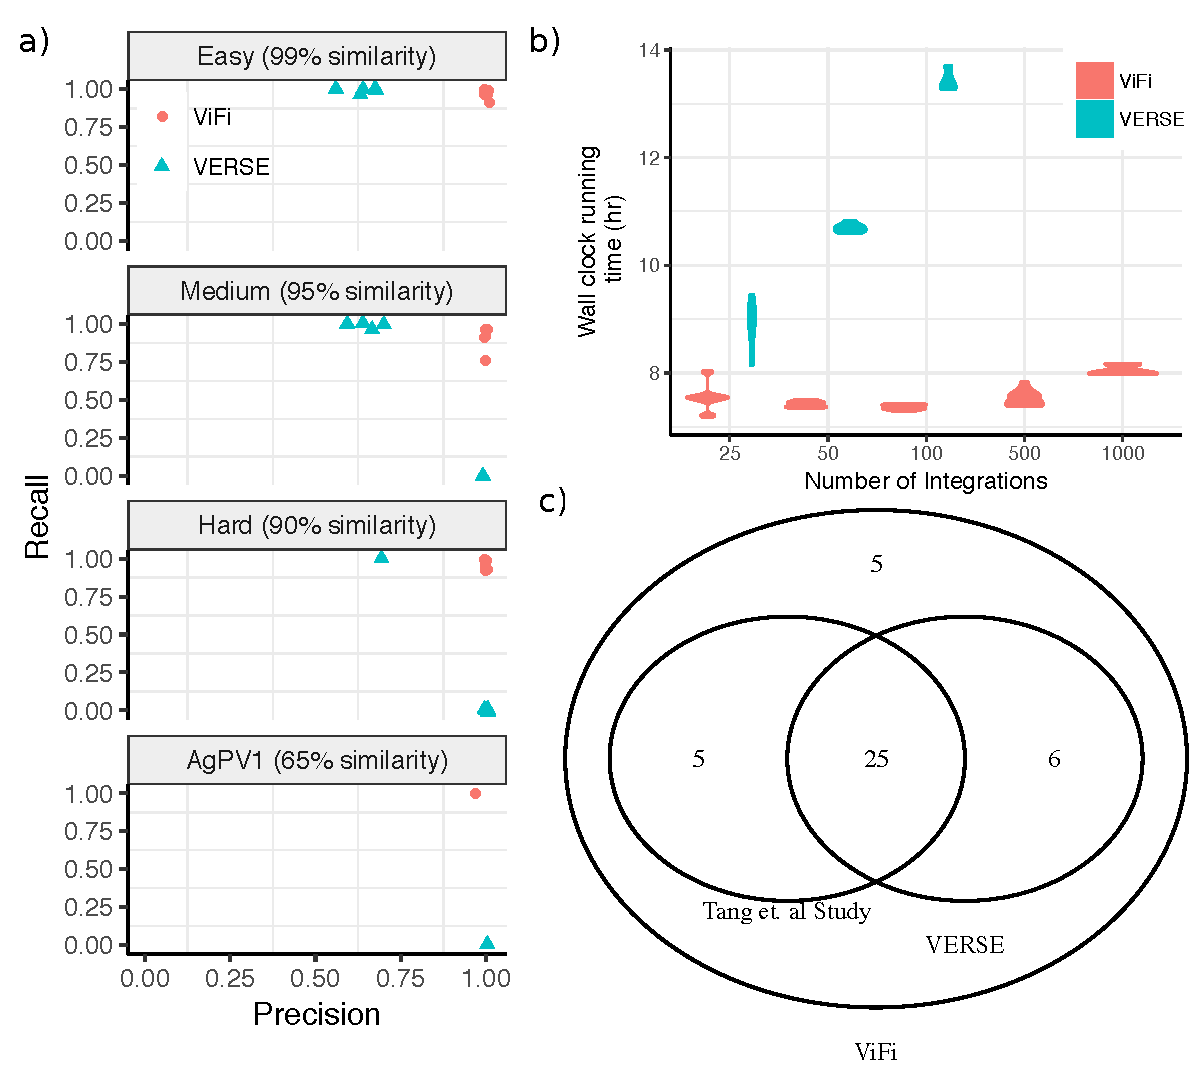
\includegraphics[width=0.90\linewidth]{results/figure1.pdf}
\caption[ViFi performance simulated datasets.]  {\label{sim_results}
  {\bf ViFi performance on simulated datasets and biological
    datasets.}  (a) The first three model conditions (easy, medium,
  and hard) vary the percent similarity of simulated HPV16 genomes to
  the reference HPV16 genome, with five replicates per simulation.
  The last model condition uses \textit{Alouatta guariba
    papillomavirus 1} (AgPV1), a PV genome not included in the set of
  viral genomes to simulate integration of a novel HPV virus.  AgPV1 is
  44\% similar to HPV16.  VERSE is unable to detect integrations or
  terminates earlier on one medium case, four hard cases, and on the
  AgPV1 dataset; we report a precision of 1 and recall of 0 on those
  cases  All datasets were simulated with 25x coverage.  (b) The mean wall clock running time
  (in hours) as a function of the number of integrations.  All methods
  were run on a machine with 24 cores for a maximum of 48 wall clock hours (1152 total core hours).  Only
  runs that report integrations were included.  (c) Venn diagram of
  the overlap of the WGS integration points with a matching mRNA event
  within 100kb reported by ViFi, VERSE, and the Tang et al. 2013 study
  on the TCGA-CESC samples with both RNA-seq and WGS sequencing
  matched pair data.}
\end{figure}


\begin{figure}[htpb]
  \centering
  %\includegraphics[width=6in]{results/{figure2}.pdf}\\
  \caption[Analyses of genomic integration sites.]  {\label{figure2}
    \textbf{Characterization of genomic integration sites and fusion
      mRNA.} \textbf{(a)} Density plot of the distance of fusion mRNA
    junction to the nearest WGS integration breakpoint.  \textbf{(b)}
    Number of annotated types covered by WGS or RNA-seq reads across
    all integration regions.  The points give
    the number of specific functional annotations (e.g. LINE) across
    all 181 integration regions in the TCGA-CESC data set that
    are partially covered by at least three reads.  Blue represents
    results from WGS data, and red represents results from RNA-seq
    data.  The violin plot show the distribution of the total number
    of specific annotations across 1,000 replicates that are partially
    covered by at least three reads, where each replicate is a
    collection of 181 randomly chosen intervals. The $p$-values of the
    observed annotation counts (Z-test) are all statistically
    significant for the RNA-seq data($p$-value $<10^{-20}$), but for the
    WGS data only the SINE elements ($p$-value $<10^{-8}$) and genes
    ($p$-value $<10^{-7}$) were enriched in a statistically significant
    manner.}
\end{figure}

\begin{figure}[htpb] \centering
  %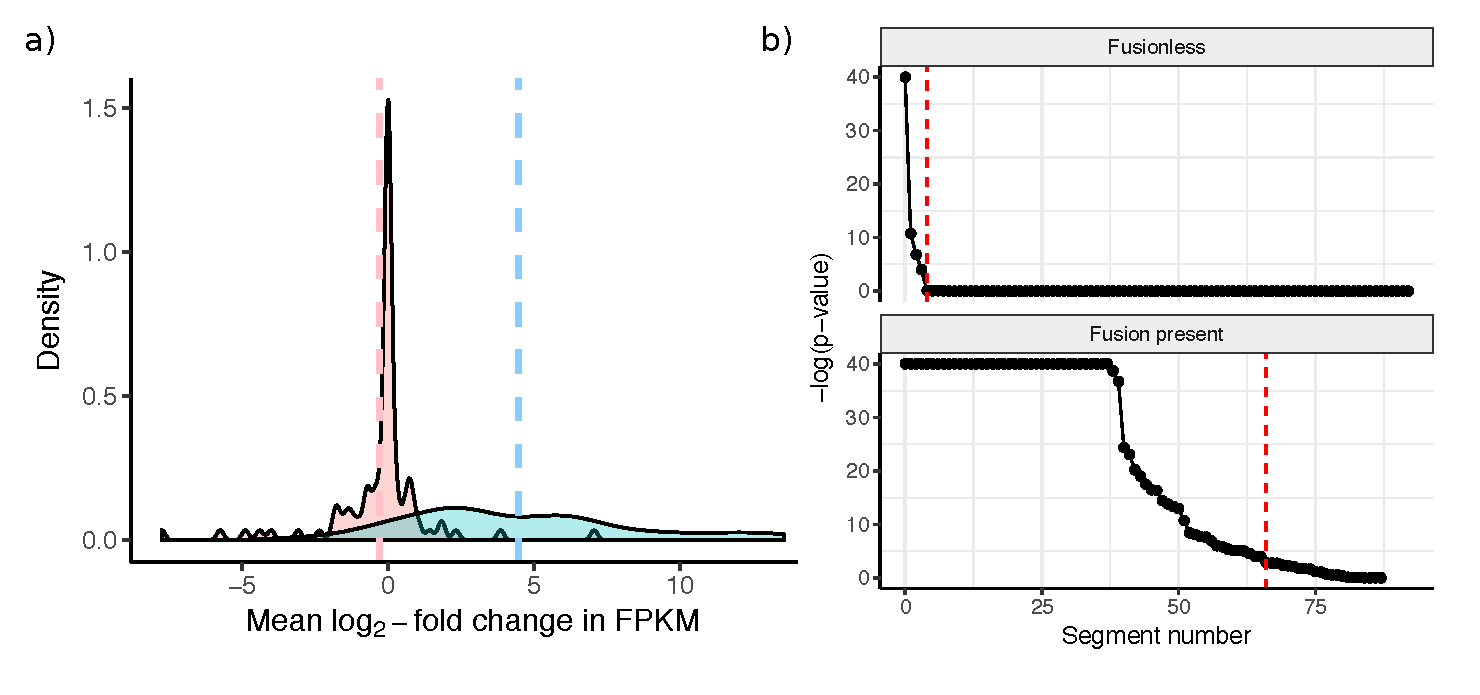
\includegraphics[width=6in]{{results/figure3}.pdf}
  \caption[Log$_2$-fold change of expression between genomic segments with
  and without integrations.]  {\label{figure_3} {\bf
        Impact of viral integration on proximal transcription.}  For each integration, we compare the expression change in the 10kb genomic interval around an integration in a sample to the mean expression change for the same 10kb genomic interval for all other samples without the integration.  \textbf{(a)}  The distribution of log$_2$-fold change in expression of human mRNA between segments with and without integrations, separated by whether the integration produces fusion mRNA or is a fusionless integration.  \textbf{(b)} The -log($p$-value) for
  expression change for integrations that produce fusion mRNA and fusionless integrations (see \textbf{Methods} for description of $p$-value computation).  The red dashed line denotes the threshold beyond which the samples do not show a significant change in expression ($p$-value $>0.05$ after FDR correction).}
\end{figure}

\begin{figure}[htpb] \centering
    %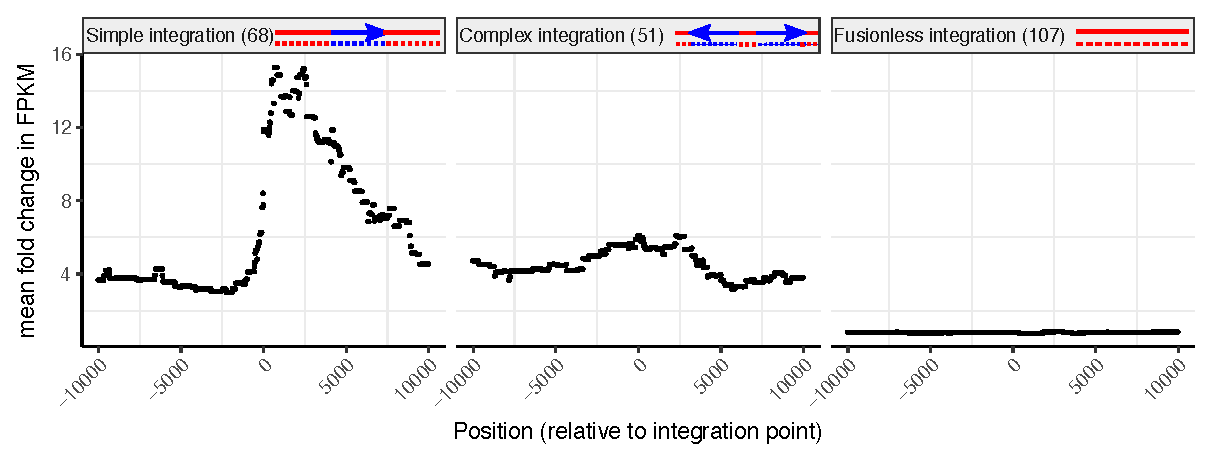
\includegraphics[width=6.1in]{{results/updown.10000}.pdf}
  \caption[Fusion reads supp.]  {\label{updown} {\small {\bf
        Expression of human segments upstream and downstream of the
        integrated viral gene}. The blue line represents
        an integrated virus, with arrow representing the direction of transcription
        of the viral genome, and the red line represents the human genome.  An integration is denoted as
      `fusionless' when it does not contain a mapped chimeric
      (viral-human mRNA); otherwise, it is denoted as `simple' when it
      is the only integration within a 10kb window, and at least 75\%
      of the chimeric paired-end reads supporting a fusion mRNA event
      are oriented in the same direction relative to the viral
      gene. All other regions are denoted `complex'. The position is
      reported relative to the integration point in the human genome,
      with negative position being upstream of the viral gene, and
      positive position being downstream of the viral gene. In total,
      there are 68 simple integrations, 51 complex integrations, and
      107 integration events with no fusion mRNA sequences. We observe
      a high increase downstream of simple integrations, in the entire
      region of complex integrations, and no increase in expression in
      fusionless integrations.}} %35,
\end{figure}

\begin{figure}[htpb]
  \centering
  %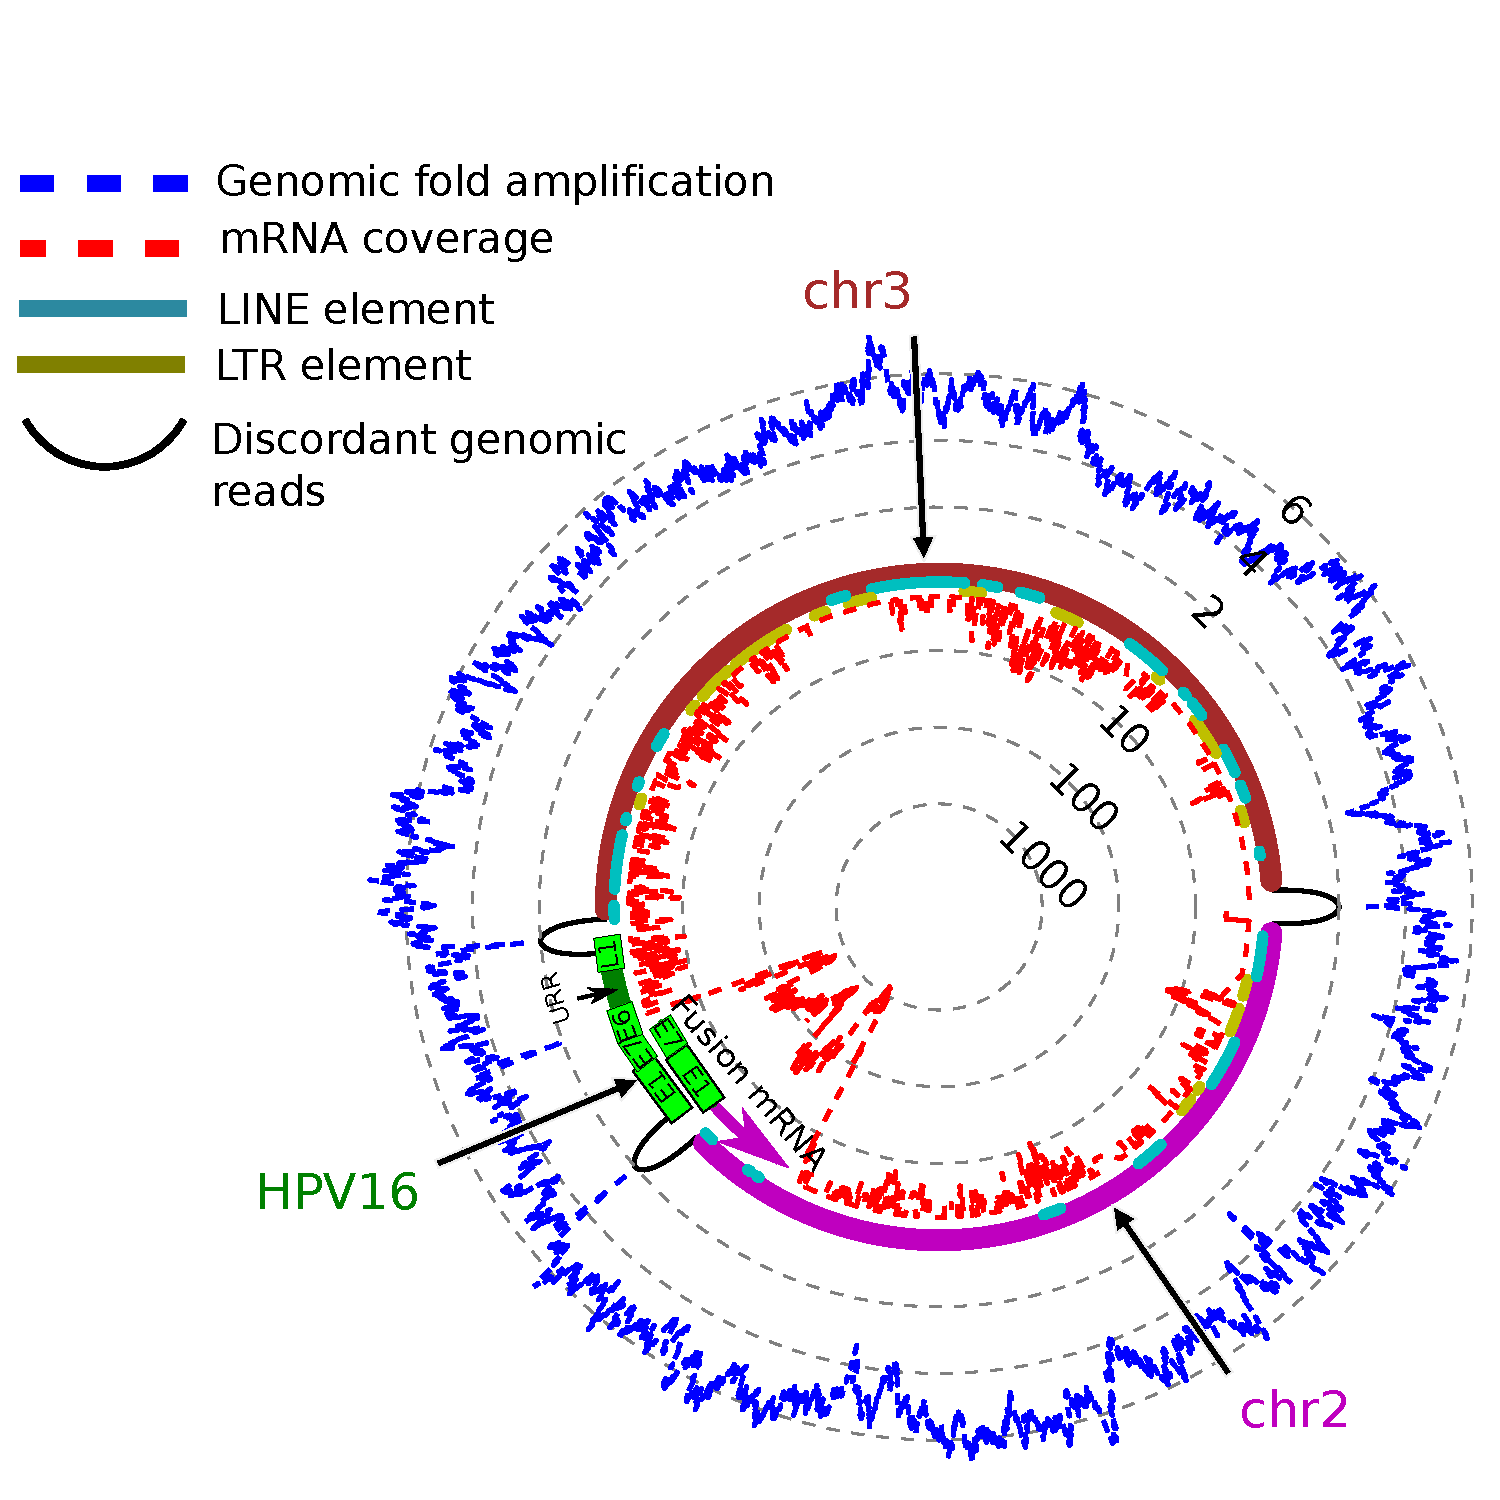
\includegraphics[width=5in]{{results/TCGA-C5-A0TN-final}.pdf}
\caption[Proposed ecDNA structure for TCGA-C5-A0TN.]
{\label{tcga_c5_a0tn}  {\bf Proposed ecDNA structure for TCGA-C5-A0TN.}  Proposed ecDNA structure for an integration from TCGA-C5-A0TN.   The joined segments are chr2:195586245-195603512, chr3:126826267-126849186, and HPV16:0-7905.  There are 235 chimeric paired-end between chr2 and HPV16, 149 discordant paired-end reads between chr2 and chr3, and 229 chimeric paired-end reads between
chr3 and HPV16.  The genomic coverage fold amplification of the region relative to the average genomic coverage of the entire genome is shown in blue, and the mRNA coverage of the region is shown red.  The FPKM fold change for the human mRNA in this region for this sample is 7200x.  LINE and LTR elements are highlighted in teal and gold.  The viral genes are highlighted in light green.  The assembled fusion transcript from this region is shown in the figure.}
\end{figure}

\begin{figure}[htpb]
  \centering
  %\includegraphics[width=8in]{{preprocess}.pdf}\\
  %\includegraphics[width= 4in]{{mapping}.pdf}
  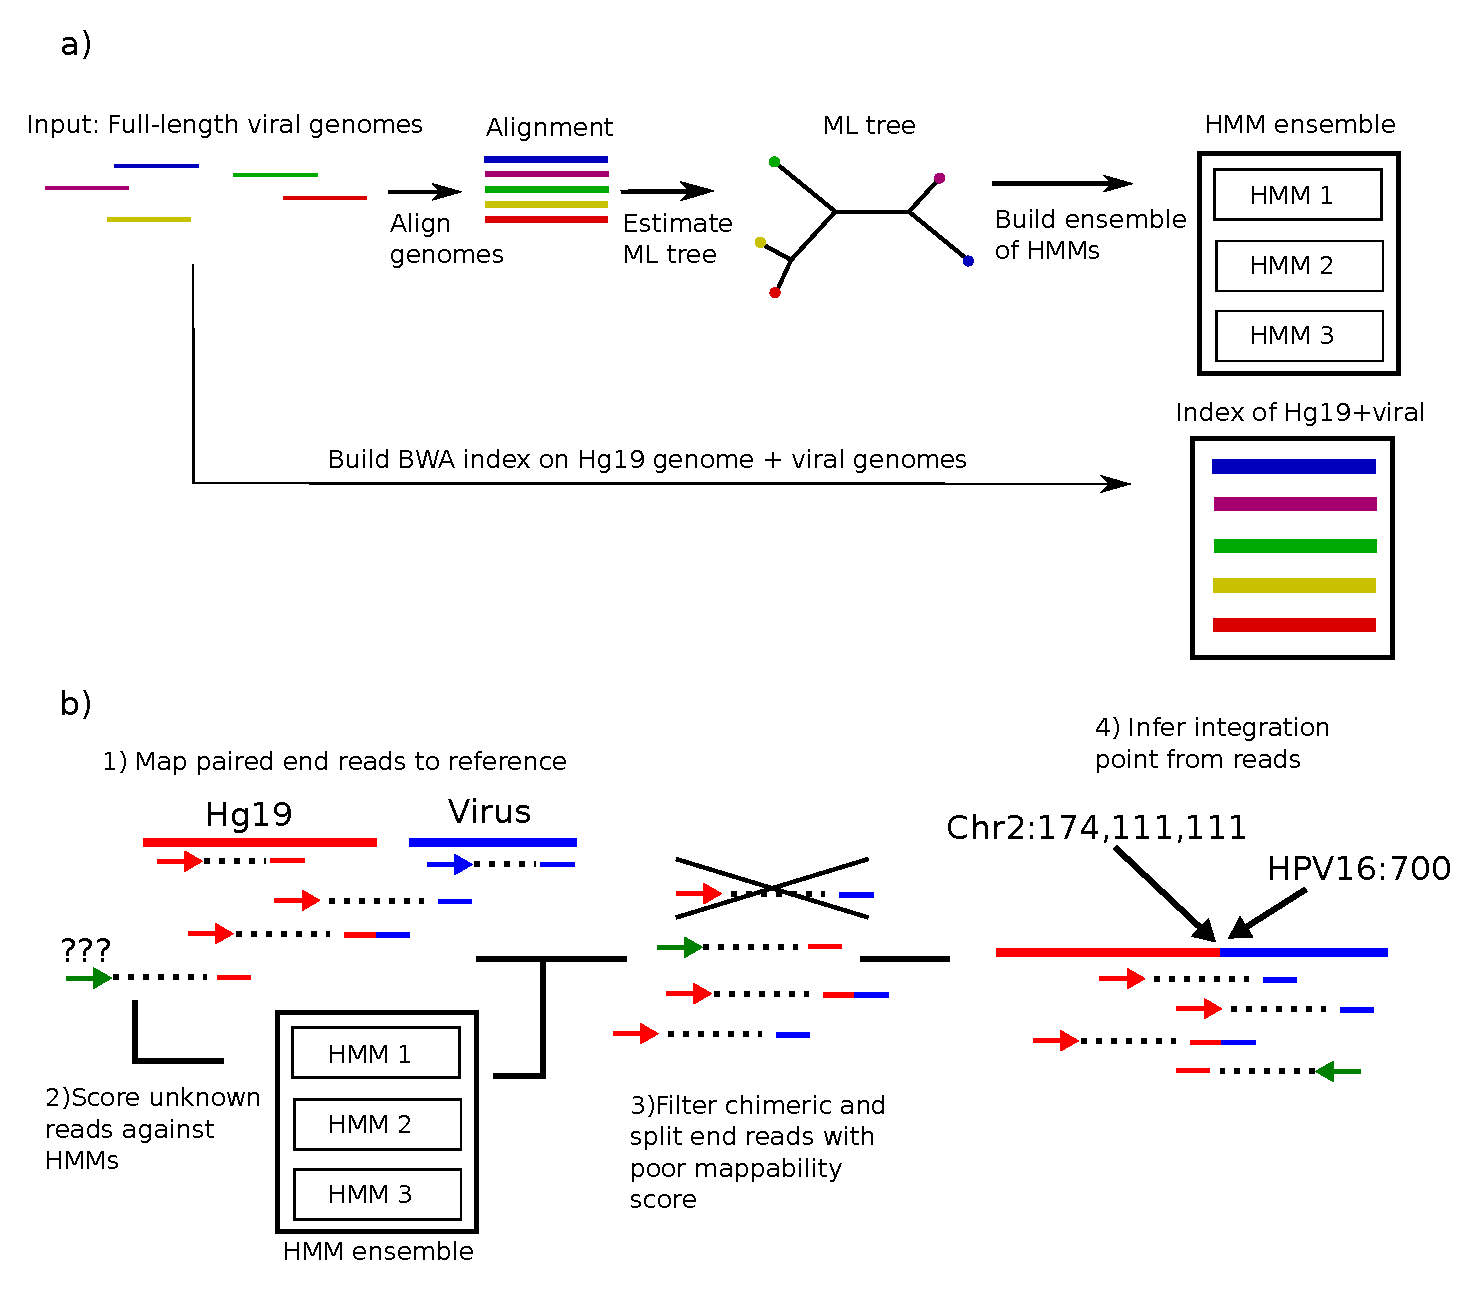
\includegraphics[width= 6in]{{results/figure6}.pdf}
\caption[Overview of integration detection process.]
{\label{flowchart}  {\bf Overview of integration detection process.}  Integration detection is split into two phases.  In the a) pre-processing step, a BWA index is created from the human reference genome and input viral genomes (Hg19+viral).  In addition, a multiple sequence alignment is estimated from the viral genomes, and an maximum likelihood tree is estimated from the alignment.  The alignment is decomposed into an ensemble of profile Hidden Markov models.  In the b) viral detection step, the paired-end reads are mapped against the Hg19+viral index.  Candidate paired-end reads are selected if, i) one end of the read maps to the human genome and the other end maps to a viral genome, or ii) one end of the read maps to the human genome and the other end scores high against the HMM ensemble.  All other reads are discarded.  The integration point is then inferred from the set of candidate reads.}
\end{figure}

\begin{figure}[htpb]
  \centering
  %\includegraphics[width=1\linewidth]{results/{ehmms}.pdf}\\
\caption[Ensemble of HMMs technique.]
{\label{ehmms}  {\bf Algorithm for generating the ensemble of HMMs.}  The input is an initial multiple sequence alignment (MSA) and a maximum likelihood (ML) tree that has been estimated for the MSA. The algorithm begins by adding the HMM built on the MSA to the ensemble. If the MSA has more than 10 sequences, the ML tree is decomposed into two subtrees by deleting the centroid edge (i.e., the edge that produces a maximally balanced split of the sequence set into two sets). The subtrees are used to generate induced alignments. HMMs are built for each induced alignment and added to the ensemble. The process iterates on those subtrees that meet the criterion for decomposition (subset size more than 10).}
\end{figure}
%%%%%%%%%%%%%%%%%%%%%%%%%%%%%%%%%%%
%%                               %%
%% Tables                        %%
%%                               %%
%%%%%%%%%%%%%%%%%%%%%%%%%%%%%%%%%%%

%% Use of \listoftables is discouraged.
%%
\section*{Tables}
\begin{table*}[htb]
\centering
\caption{\textbf{Overview of datasets}.  We provide an overview of the datasets used throughout this study.  }
\label{table:data}
\begin{tabular}{|l|l|l|r|r|}
\hline
\multicolumn{1}{|c|}{Dataset name} & \multicolumn{1}{|c|}{Type} & \multicolumn{1}{|c|}{Source} & \multicolumn{1}{|c|}{Number of} & \multicolumn{1}{|c|}{Source} \\ 
 &  &  & \multicolumn{1}{|c|}{samples} & \\ \hline 
HPV-Sim & WGS &Simulated& 16 & This study \\ \hline
HCC-WGS & WGS & Biological&20 & ~\cite{Sung2012}\\ \hline%~\cite{Sung2012} \\ \hline
HCC-RNA & RNA-seq & Biological&6 & ~\cite{Lau2014} \\ \hline%~\cite{Lau2014} \\ \hline
TCGA-CESC & WGS and RNA-seq &Biological& 68 & ~\cite{TCGA} \\ \hline %~\cite{TCGA} \\ \hline 
\end{tabular}
\end{table*}

%%%%%%%%%%%%%%%%%%%%%%%%%%%%%%%%%%%
%%                               %%
%% Additional Files              %%
%%                               %%
%%%%%%%%%%%%%%%%%%%%%%%%%%%%%%%%%%%

\section*{Additional Files}
  \subsection*{\textbf{Additional file 1} --- supplement.pdf}
    This file contains supplementary figures, commands needed to re-run the analyses, and information on 
    debugging VERSE and ViralFusionSeq.
    
  \subsection*{\textbf{Additional file 2} --- Supplementary Tables.xlsx}
    This file contains the supplementary tables for this study.  Supplementary Table 1 contains the reference viral genomes used in the study.  Supplementary Table 2 contains the simulation accuracy scores per replicate for ViFi and VERSE.  Supplementary Table 3 contains the list of genomic integrations and fusion mRNA found by ViFi.  Supplementary Table 4 contains the normalized transcription expression for the TCGA-CESC data for the genomic integration regions containing integrations.  Supplementary Table 5 contains the list of TCGA-CESC samples used in the study.  Supplementary Table 6 contains the list of samples used from the Sung et al. 2012 study.


\end{backmatter}
\end{document}
